\textbf{COLUNI 2025 -- Questão 27}\par\medskip O sangue é um tipo de tecido essencial para a circulação de substâncias em alguns animais, desempenhando funções como o transporte de oxigênio, nutrientes e hormônios. As características do tecido sanguíneo podem variar entre os diferentes grupos de vertebrados.

% COLUNI-AUTO-FIGURES-BEGIN
\begin{figure}[htbp]
\centering
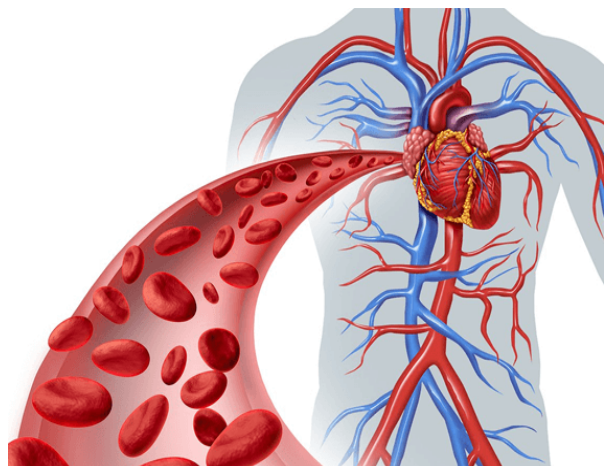
\includegraphics[width=0.55\linewidth]{static/simulados/coluni/figuras/2025/questao-27/figura-1.png}
\end{figure}
% COLUNI-AUTO-FIGURES-END
\noindent Disponível em: https://brasilescola.uol.com.br/biologia/hemacias.htm. Acesso em: 03 set. 2024.

Com base nessas diferenças, assinale a alternativa que corresponde CORRETAMENTE às características deste tecido em mamíferos:
\begin{enumerate}
\item Hemácias nucleadas e matriz extracelular fluida.
\item Hemácias anucleadas e matriz extracelular sólida.
\item Hemácias nucleadas e matriz extracelular sólida.
\item Hemácias anucleadas e matriz extracelular fluida.
\end{enumerate}
